% Options for packages loaded elsewhere
\PassOptionsToPackage{unicode}{hyperref}
\PassOptionsToPackage{hyphens}{url}
\documentclass[
]{ltjsarticle}
\usepackage{xcolor}
\usepackage[margin=20mm]{geometry}
\usepackage{amsmath,amssymb}
\setcounter{secnumdepth}{-\maxdimen} % remove section numbering
\usepackage{iftex}
\ifPDFTeX
  \usepackage[T1]{fontenc}
  \usepackage[utf8]{inputenc}
  \usepackage{textcomp} % provide euro and other symbols
\else % if luatex or xetex
  \usepackage{unicode-math} % this also loads fontspec
  \defaultfontfeatures{Scale=MatchLowercase}
  \defaultfontfeatures[\rmfamily]{Ligatures=TeX,Scale=1}
\fi
\usepackage{lmodern}
\ifPDFTeX\else
  % xetex/luatex font selection
\fi
% Use upquote if available, for straight quotes in verbatim environments
\IfFileExists{upquote.sty}{\usepackage{upquote}}{}
\IfFileExists{microtype.sty}{% use microtype if available
  \usepackage[]{microtype}
  \UseMicrotypeSet[protrusion]{basicmath} % disable protrusion for tt fonts
}{}
\makeatletter
\@ifundefined{KOMAClassName}{% if non-KOMA class
  \IfFileExists{parskip.sty}{%
    \usepackage{parskip}
  }{% else
    \setlength{\parindent}{0pt}
    \setlength{\parskip}{6pt plus 2pt minus 1pt}}
}{% if KOMA class
  \KOMAoptions{parskip=half}}
\makeatother
\usepackage{graphicx}
\makeatletter
\newsavebox\pandoc@box
\newcommand*\pandocbounded[1]{% scales image to fit in text height/width
  \sbox\pandoc@box{#1}%
  \Gscale@div\@tempa{\textheight}{\dimexpr\ht\pandoc@box+\dp\pandoc@box\relax}%
  \Gscale@div\@tempb{\linewidth}{\wd\pandoc@box}%
  \ifdim\@tempb\p@<\@tempa\p@\let\@tempa\@tempb\fi% select the smaller of both
  \ifdim\@tempa\p@<\p@\scalebox{\@tempa}{\usebox\pandoc@box}%
  \else\usebox{\pandoc@box}%
  \fi%
}
% Set default figure placement to htbp
\def\fps@figure{htbp}
\makeatother
\setlength{\emergencystretch}{3em} % prevent overfull lines
\providecommand{\tightlist}{%
  \setlength{\itemsep}{0pt}\setlength{\parskip}{0pt}}
\usepackage{bookmark}
\IfFileExists{xurl.sty}{\usepackage{xurl}}{} % add URL line breaks if available
\urlstyle{same}
\hypersetup{
  hidelinks,
  pdfcreator={LaTeX via pandoc}}

\author{}
\date{}

\begin{document}

\section{Linear Simplexification by Square-Quantity Readout and a
Dimension-wise Organization of Curvature-Correction
Candidates}\label{linear-simplexification-by-square-quantity-readout-and-a-dimension-wise-organization-of-curvature-correction-candidates}

\textbf{Subtitle}: The positive square map, elementary motion forms, and
correction candidates in length, area, and volume

\textbf{Author}: Noriaki Kihara\\
\textbf{Version}: v0.1-r1 (reflecting ChatGPT review and author
comments)\\
\textbf{Date}: 2026-06-21\\
\textbf{DOI}: Version 10.5281/zenodo.20785540 (this version) / Concept
10.5281/zenodo.20785539 (cite this; always resolves to the latest
version)\\
\textbf{Zenodo}: https://zenodo.org/records/20785540\\
\textbf{Position}: First draft as an observational and organizing paper.
The possible originality does not lie in the square map itself, but in
the way the square-quantity readout can be placed side by side with the
dimension-wise results of the self-referenced Paper 0, thereby
organizing where curvature-correction candidates first become relevant
among length, area, and volume. This paper does not claim to prove
physical laws, assert observational facts, or replace established
physics.\\
\textbf{Self-reference}: Noriaki Kihara, ``Paper 0: Distortion of the
Geodesic Unit Cell in Positively-Curved Constant-Curvature Space'',
v1.4.

\begin{center}\rule{0.5\linewidth}{0.5pt}\end{center}

\subsection{Abstract}\label{abstract}

This paper formulates, using only elementary geometry and elementary
algebra, the following fact. If the square quantities

\[
X_i=x_i^2
\]

are read as the basic variables on the positive real domain, then the
curved sum-of-squares constraint

\[
\sum_i x_i^2=E
\]

is read, in square-quantity space, as the linear constraint

\[
\sum_i X_i=E.
\]

This fact itself has known relatives, for example the square-root
representation connecting a probability simplex with the positive
orthant of a sphere in information geometry. Therefore, this paper does
not claim the correspondence between the simplex and the positive
spherical orthant as a new theorem.

The aim of this paper is to place this square-root correspondence, which
is close to known constructions, not as a geometry of probability
densities but as a general ``square-quantity readout'', and then to
observe at which geometric dimension a curvature-correction candidate
first becomes relevant. The square-quantity readout does not make
curvature disappear. Rather, one sees a branching: no correction
candidate appears in relations closed by length alone, while the
area-correction coefficient

\[
k_s(R)
\]

from the self-referenced Paper 0 appears as a test candidate when a
two-dimensional area quantity first enters.

More concretely, first we confirm that the positive square map sends
sum-of-squares constraints such as a circular arc or a spherical octant
exactly to linear constraints such as a line segment or a triangular
simplex. Second, we place simple equations on the square-quantity side
and see that, under positive square-root readout, equations isomorphic
to uniform-motion and uniformly-accelerated-motion forms are obtained.
Third, even if masses and conservation laws are externally imposed, as
in a two-body collision, no area correction appears as long as the
situation is closed in one dimension. Fourth, a centrifugal-type model,
in which tangential and radial directions appear simultaneously, is
treated as the first natural test example in which an area quantity
appears.

This paper states the above as observations and elementary statements in
geometry and algebra. Equations from classical physics are used only as
examples for asking: if a known form is placed on the square-quantity
side or on the square-root side, which geometric dimension of correction
becomes relevant? They are not used as derivations of physical laws.

\begin{center}\rule{0.5\linewidth}{0.5pt}\end{center}

\subsection{0. What This Paper Claims and Does Not
Claim}\label{what-this-paper-claims-and-does-not-claim}

\subsubsection{0.1 Claims}\label{claims}

The claims of this paper are limited to the following.

\begin{enumerate}
\def\labelenumi{\arabic{enumi}.}
\item
  On the positive domain, the square map

  \[
  \Phi:(x_1,\ldots,x_n)\mapsto (X_1,\ldots,X_n)=(x_1^2,\ldots,x_n^2)
  \]

  maps a sum-of-squares constraint to a linear simplex constraint.
\item
  Its inverse is the positive square-root map

  \[
  \Psi:(X_1,\ldots,X_n)\mapsto (\sqrt{X_1},\ldots,\sqrt{X_n}),
  \]

  and the correspondence is one-to-one in the interior domains
  \(x_i>0\), \(X_i>0\).
\item
  If simple equations such as

  \[
  X=A T,\qquad X=\frac{1}{2} B T^2
  \]

  are placed on the square-quantity side, then positive square-root
  readout gives

  \[
  x=\sqrt{A}\,t,\qquad x=\sqrt{B/2}\,t^2.
  \]
\item
  According to the self-referenced Paper 0, a geodesic edge length in a
  constant-curvature space is not distorted by the construction, while
  two-dimensional area is distorted. Hence a branching rule arises: no
  area correction is inserted into a one-dimensional relation closed by
  length alone, and \(k_s(R)\) first becomes a candidate when an area
  cell spanned by two directions appears.
\item
  A centrifugal-type model is treated as the first natural test example
  in which an area quantity appears. The insertion of \(k_s(R)\)
  proposed there is not a physical law uniquely derived from geometry,
  but a model readout under the assumptions of constant curvature and
  uniform correction.
\end{enumerate}

\subsubsection{0.2 Non-claims}\label{non-claims}

This paper does not claim the following.

\begin{itemize}
\tightlist
\item
  It does not claim to prove physical laws.
\item
  It does not claim to replace classical mechanics, relativity, or
  quantum theory.
\item
  It does not identify \(X_i\) with a particular physical quantity such
  as probability, energy, mass, or time.
\item
  It does not claim that the square map is an isometry as a metric map.
\item
  It does not claim that a curved space itself disappears into a flat
  space.
\item
  It does not claim that inserting \(k_s(R)\) into a centrifugal-type
  equation is uniquely derived as a law of mechanics.
\item
  It does not claim that the non-isometry of the square map is the cause
  of \(k_s(R)\).
\item
  It does not identify the metric distortion of the square map with the
  geodesic-square area excess of the self-referenced Paper 0.
\item
  It does not reject Riemannian geometry or local differential geometry.
\end{itemize}

When this paper says that a relation is ``read as flat'', it means only
that the constraint

\[
\sum_i x_i^2=E
\]

becomes, on the square-quantity side, the affine linear equation

\[
\sum_i X_i=E.
\]

This is not an identity of metrics, but an algebraic simplification in
the readout coordinates.

\subsubsection{0.3 Precise Position of This
Paper}\label{precise-position-of-this-paper}

This paper is not an alternative theory to Riemannian geometry for
general continuous systems with local curvature. It restricts the
setting to constant-curvature spaces with a uniform curvature radius,
and to cases where geodesic unit cells can be considered.

Under this restriction, the question is what can be read using only
elementary geometry and elementary algebra. The self-referenced Paper 0
studied how edge length, vertex angle, area, and volume change with
respect to the curvature radius \(R\). As a sequel, the present paper
asks, within the square-quantity readout, which kinds of equations are
closed by length alone and which kinds require a two-dimensional area
cell.

Thus the central observation is not that curvature disappears. The
central observation is the dimension-wise organization that no
area-correction candidate appears in relations closed by length alone,
while a correction candidate first appears when an area quantity is
involved. This is a juxtaposition of several independent geometric
facts, not a claim that \(k_s(R)\) is causally derived from the
non-isometry of the square map.

\begin{center}\rule{0.5\linewidth}{0.5pt}\end{center}

\subsection{1. The Positive Square Map}\label{the-positive-square-map}

\subsubsection{1.1 The Two-Dimensional
Case}\label{the-two-dimensional-case}

First consider two dimensions. In the positive quadrant

\[
x\ge 0,\qquad y\ge 0,
\]

take the unit circular arc

\[
x^2+y^2=1.
\]

Set

\[
X=x^2,\qquad Y=y^2.
\]

Then immediately

\[
X+Y=1.
\]

Thus a point on the positive circular arc is read, on the
square-quantity side, as a point on a straight line simplex.

\begin{figure}
\centering
\pandocbounded{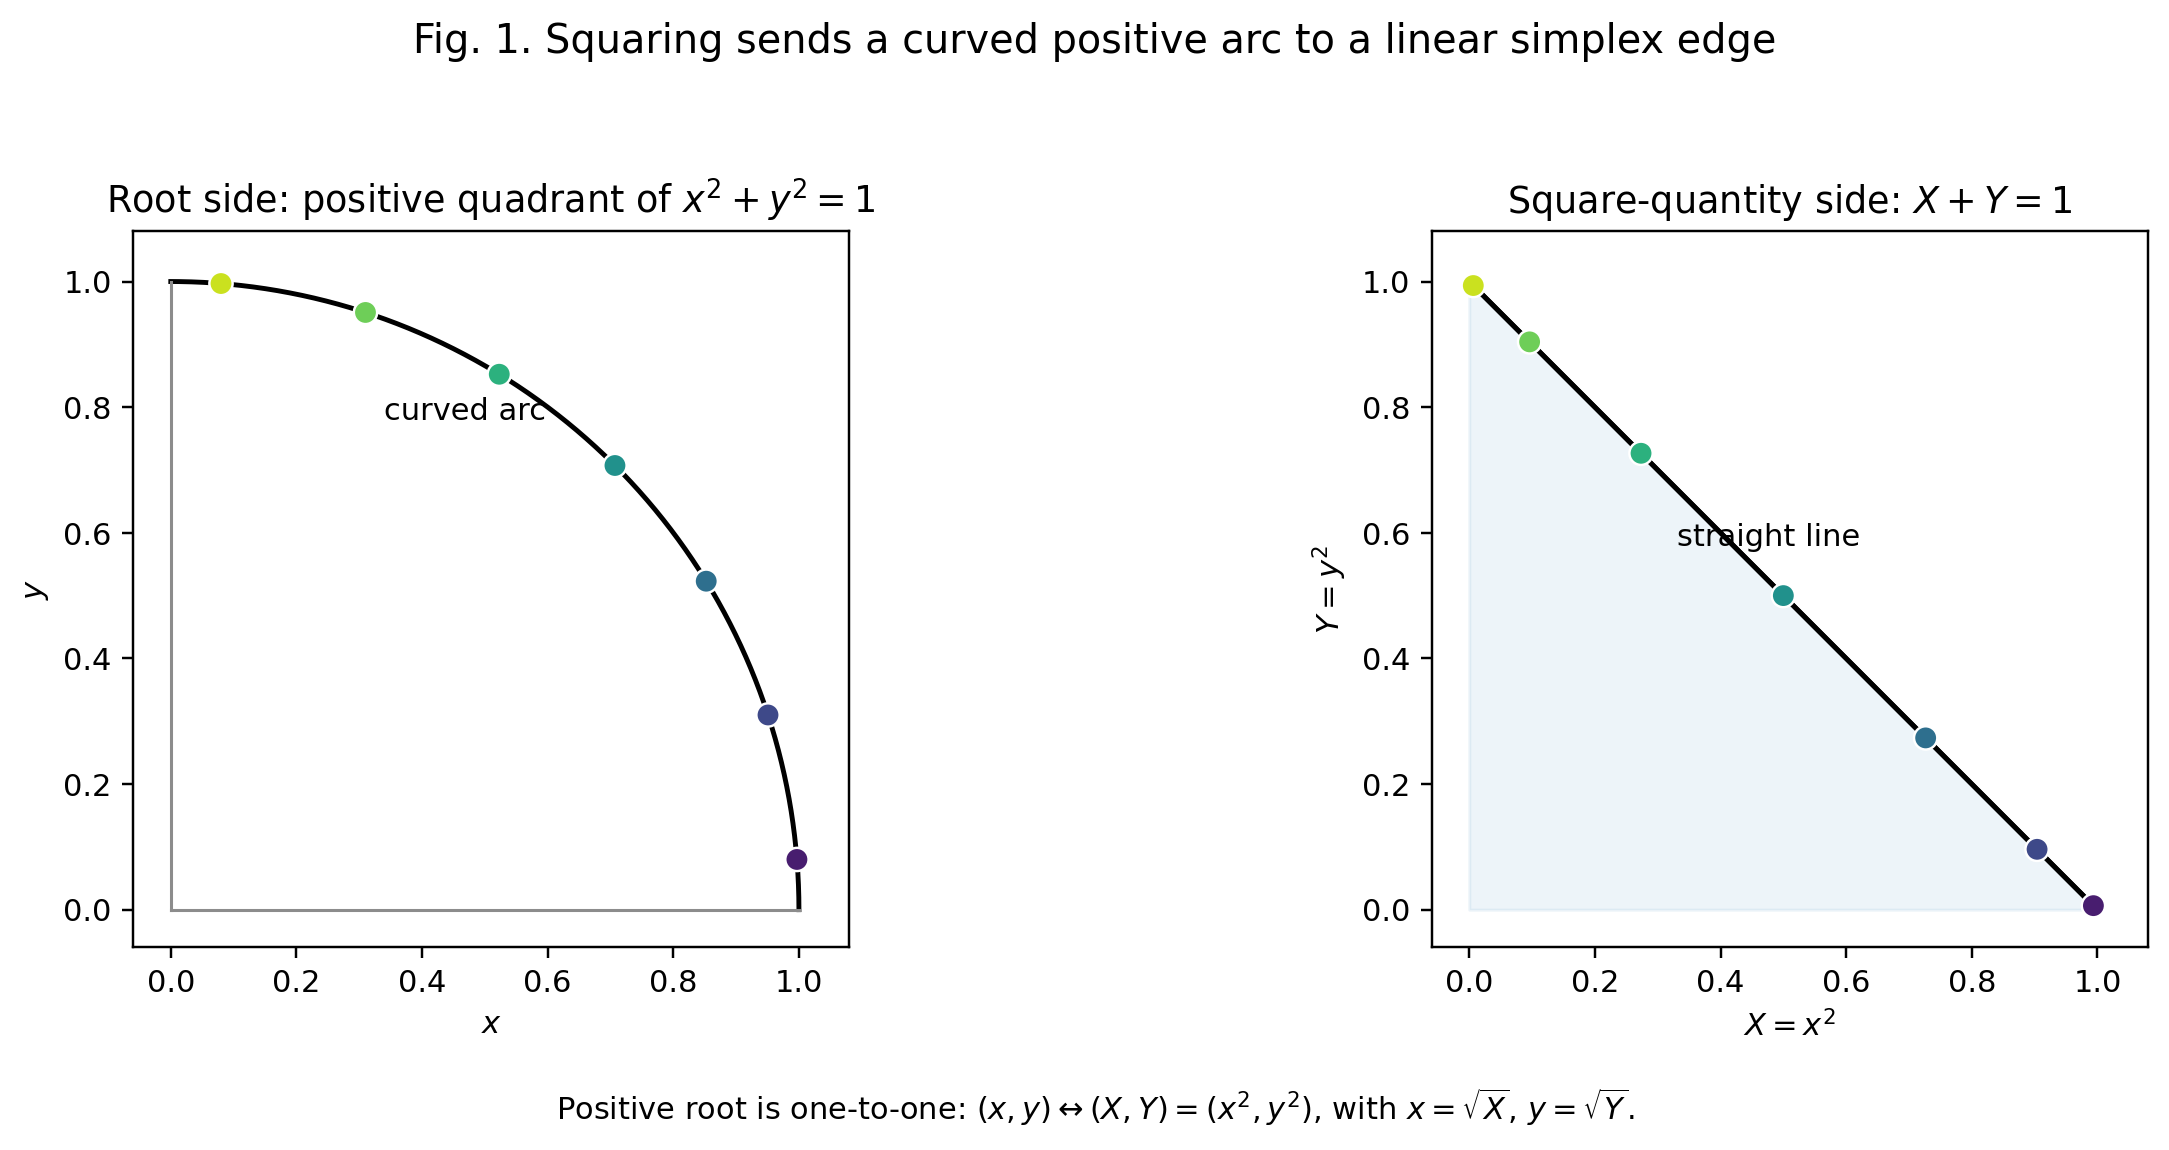
\includegraphics[keepaspectratio,alt={Fig. 1}]{figures/fig01_2d_square_map.png}}
\caption{Fig. 1}
\end{figure}

\textbf{Figure 1.} The positive circular arc \(x^2+y^2=1\) is read on
the square-quantity side as the line simplex \(X+Y=1\).

This is not an approximation. For example, if

\[
(x,y)=\left(\frac{3}{5},\frac{4}{5}\right),
\]

then

\[
(X,Y)=\left(\frac{9}{25},\frac{16}{25}\right),
\]

and indeed

\[
\frac{9}{25}+\frac{16}{25}=1.
\]

Conversely, if

\[
(X,Y)=\left(\frac{9}{25},\frac{16}{25}\right)
\]

is given on the square-quantity side, taking positive square roots gives

\[
(x,y)=\left(\frac{3}{5},\frac{4}{5}\right).
\]

The restriction to the positive domain is important. If signs are
allowed, the same value \(X=x^2\) returns both \(x\) and \(-x\). In this
paper, in order to make the square-root readout unique, we basically
work on the positive domain.

\subsubsection{1.2 General Dimension}\label{general-dimension}

The same statement holds in arbitrary dimension.

On the positive domain

\[
x_i\ge 0\qquad (i=1,\ldots,n),
\]

consider the sum-of-squares constraint

\[
S_E^{n-1,+}
=
\left\{
(x_1,\ldots,x_n)\mid \sum_{i=1}^{n}x_i^2=E,\ x_i\ge 0
\right\}.
\]

On the square-quantity side, set

\[
X_i=x_i^2
\]

and consider

\[
P_E^{n-1}
=
\left\{
(X_1,\ldots,X_n)\mid \sum_{i=1}^{n}X_i=E,\ X_i\ge 0
\right\}.
\]

Then

\[
\Phi:S_E^{n-1,+}\to P_E^{n-1},\qquad
\Phi(x_1,\ldots,x_n)=(x_1^2,\ldots,x_n^2)
\]

is a one-to-one correspondence, and its inverse is

\[
\Psi:P_E^{n-1}\to S_E^{n-1,+},\qquad
\Psi(X_1,\ldots,X_n)=(\sqrt{X_1},\ldots,\sqrt{X_n}).
\]

\textbf{Proof.}\\
If \((x_1,\ldots,x_n)\in S_E^{n-1,+}\), then each \(X_i=x_i^2\) is
nonnegative and

\[
\sum_i X_i=\sum_i x_i^2=E,
\]

so \(\Phi(x)\in P_E^{n-1}\).

Conversely, if \((X_1,\ldots,X_n)\in P_E^{n-1}\), then each \(X_i\ge0\),
so \(\sqrt{X_i}\) is defined, and

\[
\sum_i (\sqrt{X_i})^2=\sum_i X_i=E.
\]

Therefore \(\Psi(X)\in S_E^{n-1,+}\).

Furthermore, on the positive domain,

\[
\Psi(\Phi(x))=(\sqrt{x_1^2},\ldots,\sqrt{x_n^2})=(x_1,\ldots,x_n),
\]

and

\[
\Phi(\Psi(X))=((\sqrt{X_1})^2,\ldots,(\sqrt{X_n})^2)=(X_1,\ldots,X_n).
\]

Hence the two maps are inverse to each other. \(\square\)

\subsubsection{1.3 The Three-Dimensional
Case}\label{the-three-dimensional-case}

In three dimensions, the positive spherical octant

\[
x^2+y^2+z^2=1,\qquad x,y,z\ge0
\]

is read on the square-quantity side as the standard two-simplex

\[
X+Y+Z=1,\qquad X,Y,Z\ge0.
\]

\begin{figure}
\centering
\pandocbounded{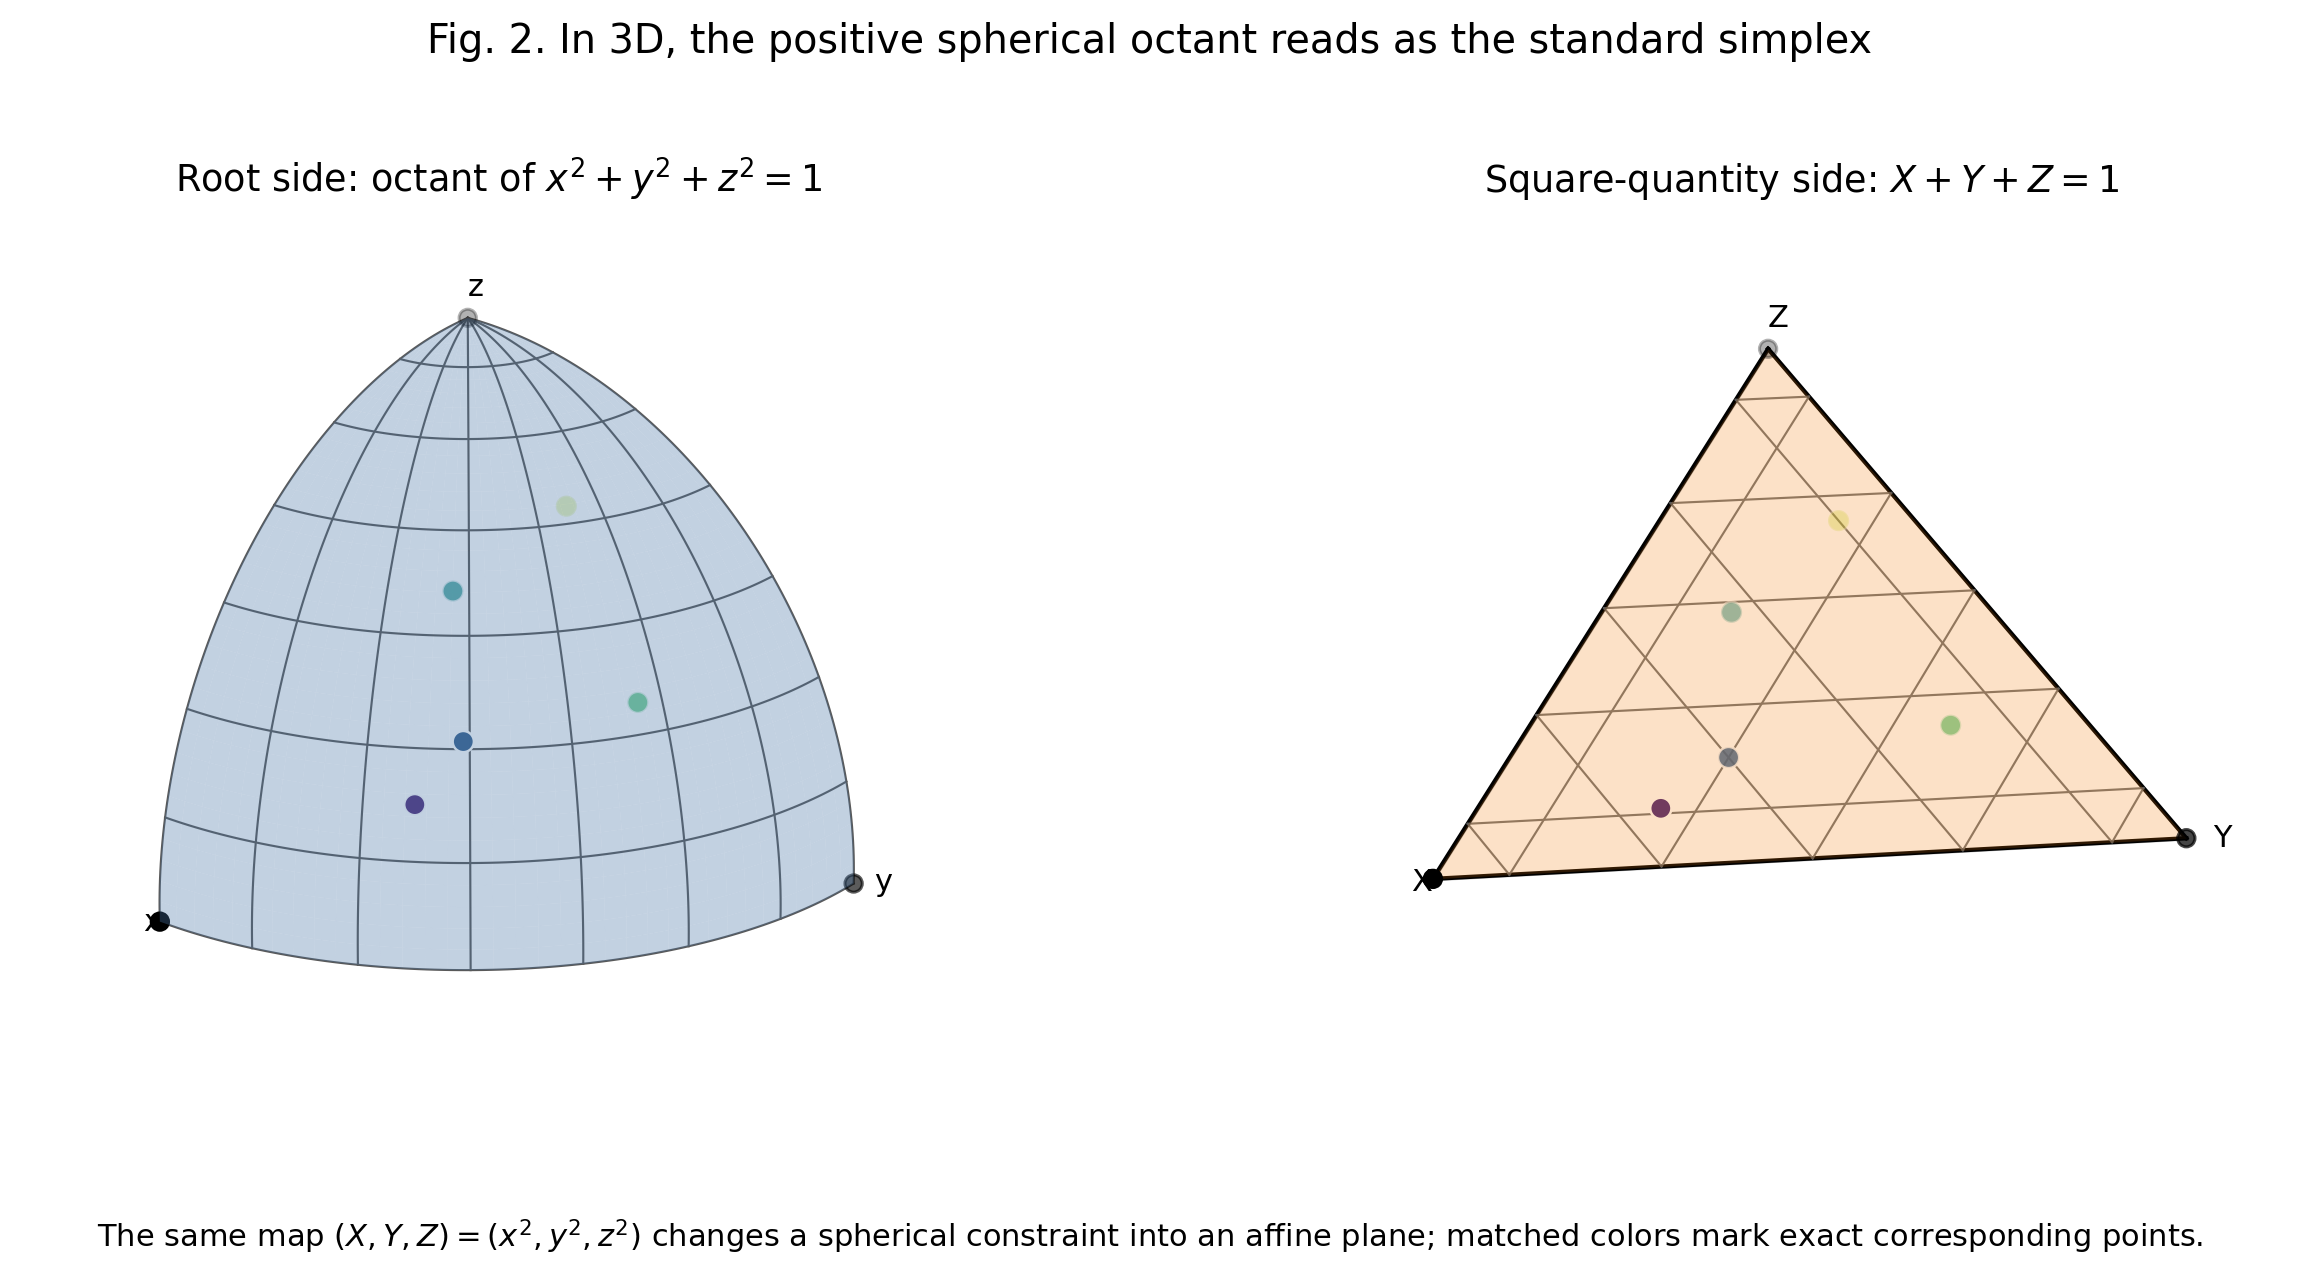
\includegraphics[keepaspectratio,alt={Fig. 2}]{figures/fig02_3d_square_map.png}}
\caption{Fig. 2}
\end{figure}

\textbf{Figure 2.} The positive spherical octant is mapped to the
standard simplex on the square-quantity side. Points of the same color
represent the same point read through the square map.

Again, the important point is that a curved constraint on the spherical
side becomes a triangle on a plane on the square-quantity side. The
figure is not schematic; it is generated from the map

\[
(X,Y,Z)=(x^2,y^2,z^2).
\]

\subsubsection{1.4 This Is Not an Isometric
Flattening}\label{this-is-not-an-isometric-flattening}

Here one must be careful. The square map is generally not an isometry.

Taking differentials gives

\[
dX_i=2x_i\,dx_i,
\]

so lengths are not preserved as they are. Therefore the intrinsic metric
of the sphere does not simply become the Euclidean metric of the plane.

The fact used in this paper is more limited.

The sum-of-squares constraint

\[
\sum_i x_i^2=E
\]

becomes, on the square-quantity side,

\[
\sum_i X_i=E.
\]

This single algebraic point is the basis of the readouts below.

\begin{center}\rule{0.5\linewidth}{0.5pt}\end{center}

\subsection{2. Placing Equations on the Square-Quantity
Side}\label{placing-equations-on-the-square-quantity-side}

\subsubsection{2.1 Basic Setting}\label{basic-setting}

We now extract two square quantities

\[
X=x^2,\qquad T=t^2.
\]

Here \(X\) and \(T\) are variables on the square-quantity side, while
\(x\) and \(t\) are their positive square-root-side variables.

This paper does not immediately identify \(T\) with physical time. It is
simply one coordinate on the square-quantity side. However, because the
resulting readout has the same form as familiar classical motion
equations, the terms ``uniform-motion form'' and
``uniformly-accelerated-motion form'' are used as comparisons.

\subsubsection{2.2 A Linear Equation Gives the Uniform-Motion
Form}\label{a-linear-equation-gives-the-uniform-motion-form}

Place

\[
X=A T
\]

on the square-quantity side, where \(A>0\) is constant.

To return to the square-root side, substitute

\[
X=x^2,\qquad T=t^2.
\]

Then

\[
x^2=A t^2.
\]

Taking the positive square root gives

\[
x=\sqrt{A}\,t.
\]

This has the same form as ordinary uniform motion

\[
x=vt.
\]

However, this paper does not call it a derivation of a physical velocity
\(v\). It only states the algebraic fact that one may read

\[
v_{\rm read}=\sqrt{A}.
\]

\subsubsection{2.3 Double-Cone-Type
Readout}\label{double-cone-type-readout}

The equation in the previous subsection may also be written as

\[
x^2-A t^2=0.
\]

If \(A=c^2\), then

\[
x^2-c^2t^2=0.
\]

Geometrically, this is a double-cone-type quadratic form, and in a
two-dimensional section it is a pair of straight lines. This paper
treats this equation not as a physical metric condition, but as a
geometric form that appears when a linear equation on the
square-quantity side is read on the square-root side.

\subsubsection{2.4 A Quadratic Equation Gives the
Uniformly-Accelerated-Motion
Form}\label{a-quadratic-equation-gives-the-uniformly-accelerated-motion-form}

Next place

\[
X=\frac{1}{2} B T^2
\]

on the square-quantity side, where \(B>0\) is constant.

Again substituting

\[
X=x^2,\qquad T=t^2
\]

gives

\[
x^2=\frac{1}{2} B t^4.
\]

Taking the positive square root gives

\[
x=\sqrt{\frac{B}{2}}\,t^2.
\]

This has the same form as ordinary uniformly accelerated motion

\[
x=\frac{1}{2} a t^2.
\]

If one compares the coefficients, then

\[
a_{\rm read}=\sqrt{2B}.
\]

Again, no physical acceleration is being proved. The statement is only
the algebraic observation that a quadratic equation on the
square-quantity side becomes the uniformly-accelerated-motion form under
positive square-root readout.

\begin{figure}
\centering
\pandocbounded{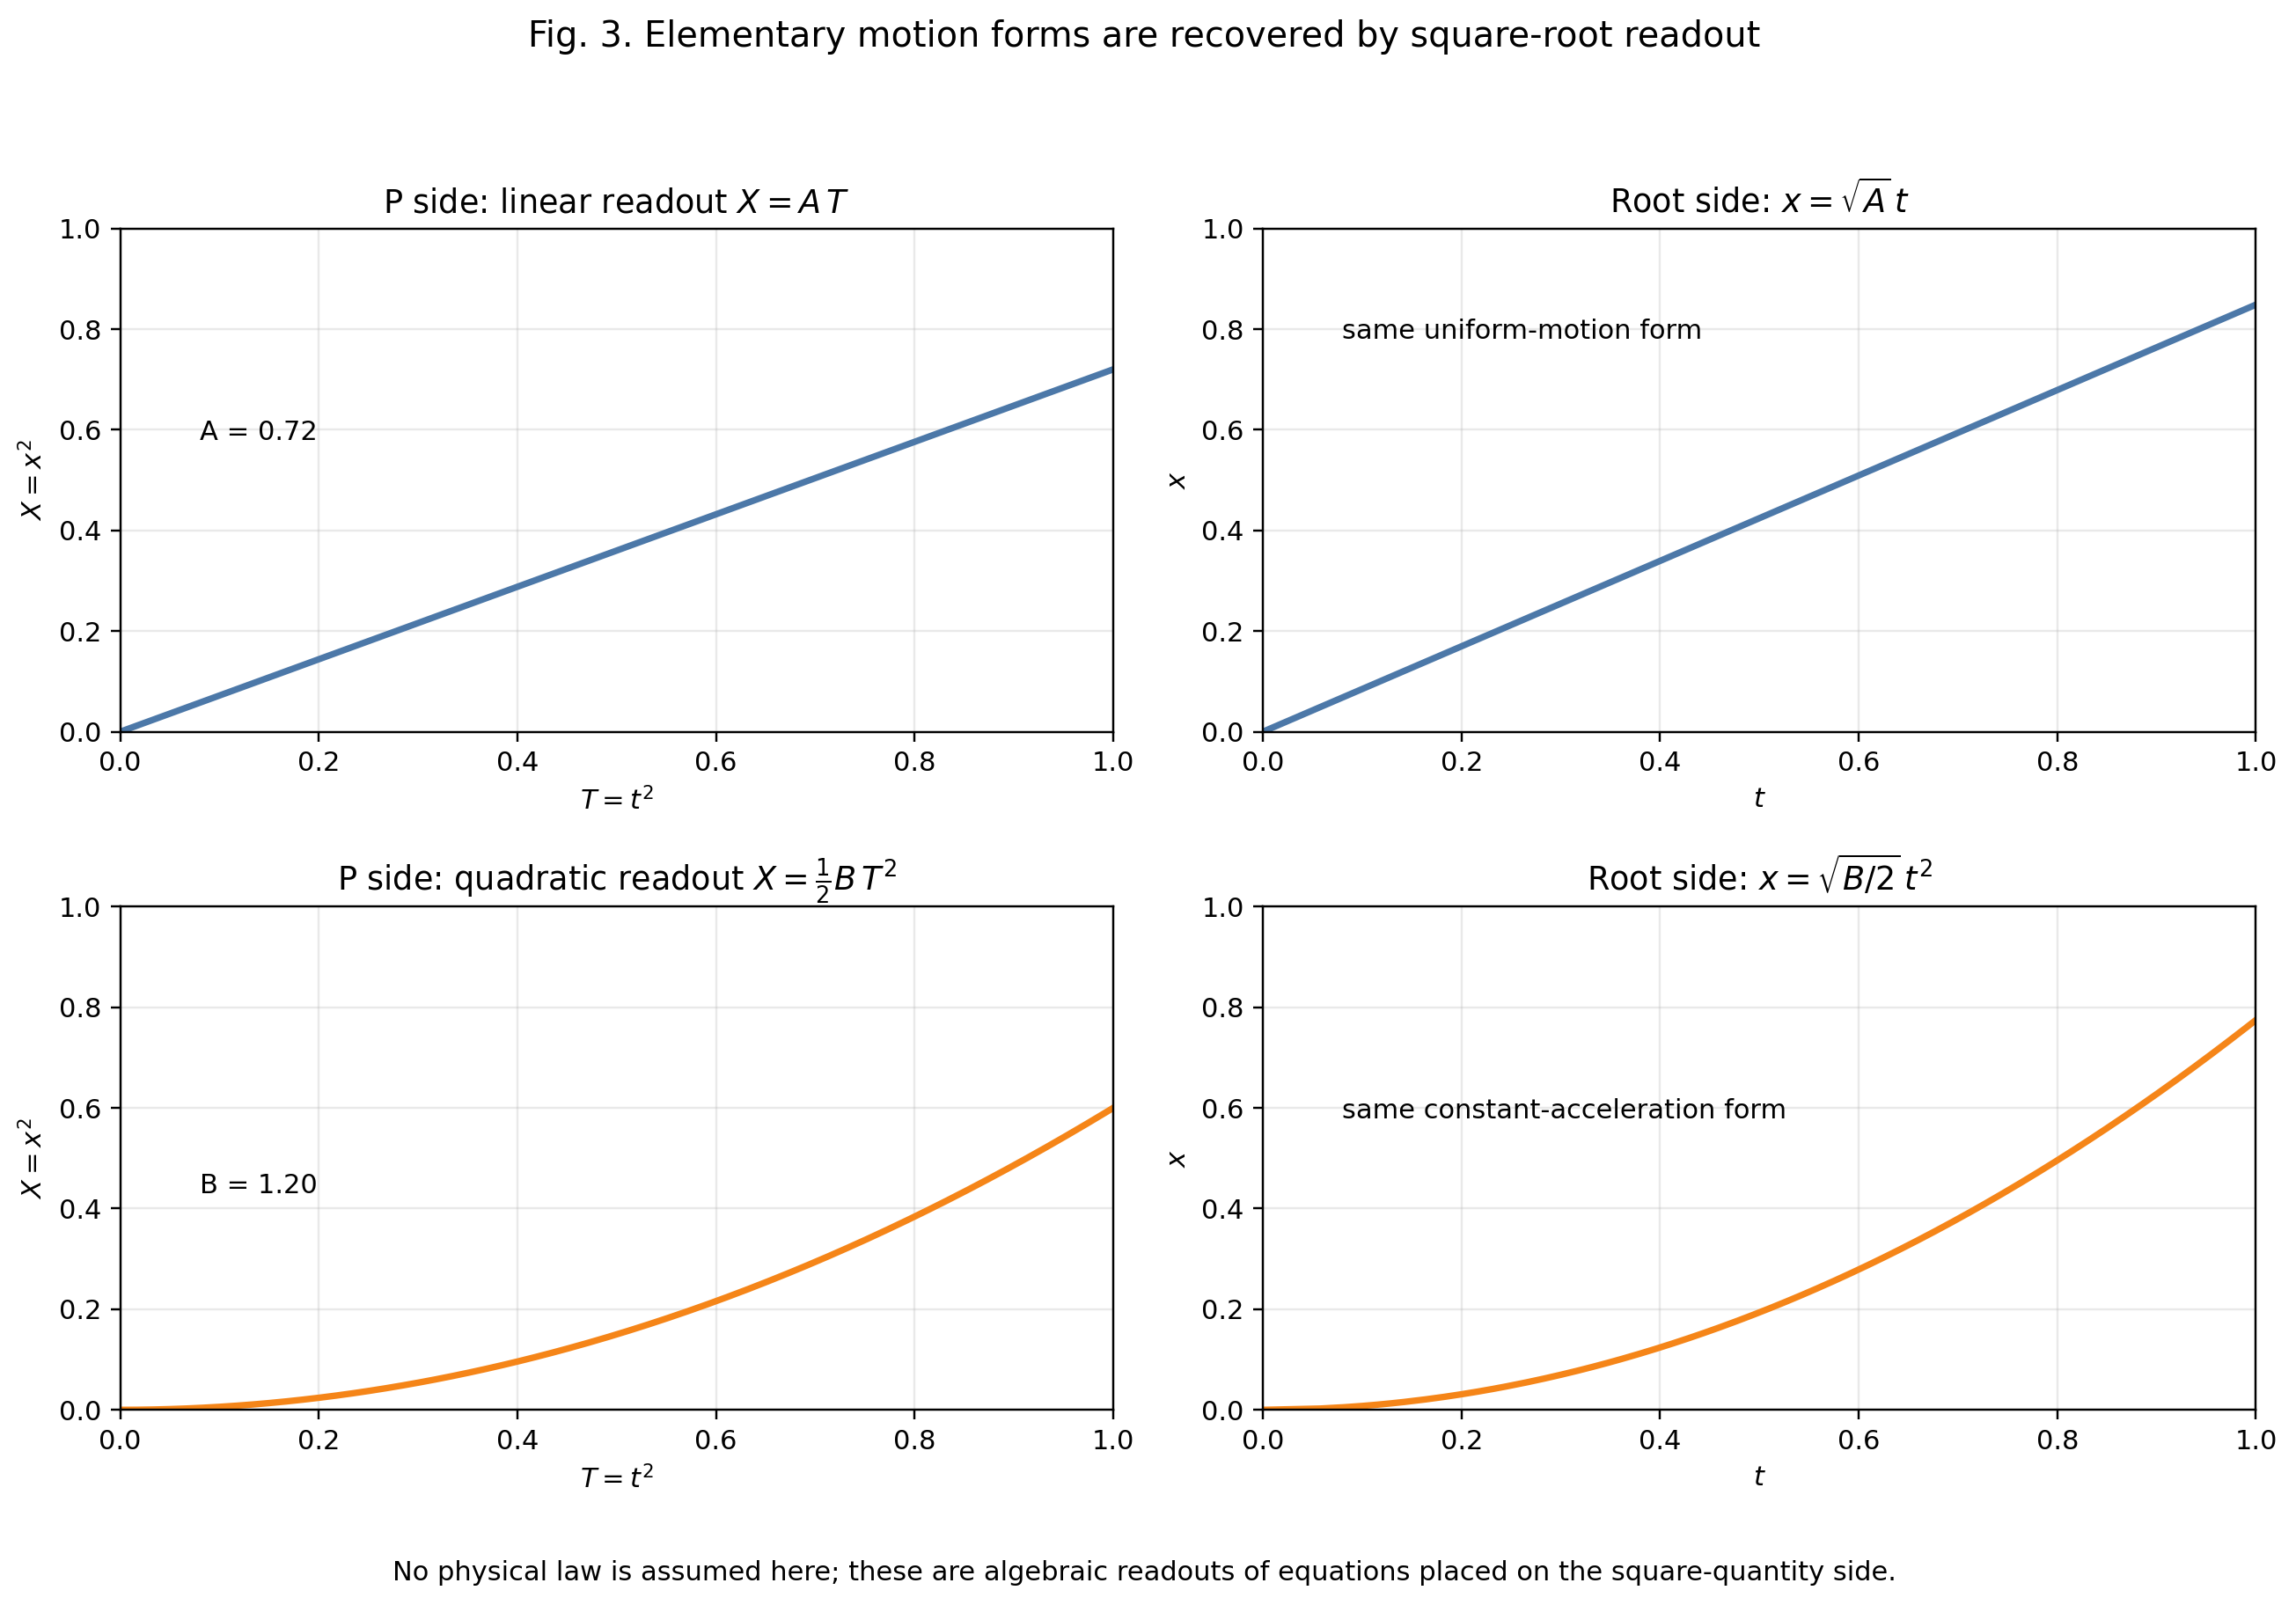
\includegraphics[keepaspectratio,alt={Fig. 3}]{figures/fig03_motion_readouts.png}}
\caption{Fig. 3}
\end{figure}

\textbf{Figure 3.} A linear equation and a quadratic equation placed on
the square-quantity side become, under positive square-root readout,
uniform-motion and uniformly-accelerated-motion forms.

\subsubsection{2.5 General Form}\label{general-form}

More generally, place

\[
X=C T^m
\]

on the square-quantity side, where \(C>0\) and \(m>0\).

Since

\[
X=x^2,\qquad T=t^2,
\]

we have

\[
x^2=C t^{2m}.
\]

Taking the positive square root gives

\[
x=\sqrt{C}\,t^m.
\]

Thus the power \(m\) on the square-quantity side appears as the same
power \(m\) on the square-root side. Only the coefficient is
square-rooted.

This is a small-looking fact, but it is important. Although \(X\) and
\(T\) are both square quantities on the square-quantity side, the
familiar power relation itself remains unchanged on the positive
square-root side.

\begin{center}\rule{0.5\linewidth}{0.5pt}\end{center}

\subsection{3. Why Curvature Correction Does Not Appear in
One-Dimensional
Equations}\label{why-curvature-correction-does-not-appear-in-one-dimensional-equations}

The self-referenced Paper 0 established the following distinction for
geodesic unit cells placed in a constant-curvature space.

\begin{itemize}
\tightlist
\item
  A geodesic edge length is exactly preserved by the construction.
\item
  Vertex angle and two-dimensional area change with the curvature radius
  \(R\).
\item
  Volume changes in a dimension-dependent way.
\end{itemize}

Moreover, Paper 0 showed that, in the small-curvature limit, the excess
coefficient of \(d\)-dimensional volume is

\[
V_d(R)=1+\frac{c_d}{R^2}+O(R^{-4}),
\qquad
c_d=\frac{d(d-1)}{12}
=\frac{\binom{d}{2}}{6}.
\]

This means that the curvature excess of \(d\)-dimensional volume can be
read as the sum of the area excesses of the \(\binom{d}{2}\) coordinate
two-planes.

From this viewpoint, the first carrier of curvature is not length but
area. In a one-dimensional relation closed by length alone, no area
correction enters.

The equations

\[
x=\sqrt{A}\,t
\]

and

\[
x=\sqrt{B/2}\,t^2
\]

from the previous section are both closed, after readout, as relations
between one \(x\) and one \(t\). No two-dimensional area cell appears.

Therefore, in the reading of this paper, there is no immediate reason to
multiply either the uniform-motion form or the
uniformly-accelerated-motion form by \(k_s(R)\).

The observation obtained here is:

\begin{quote}
Whether a curvature correction appears depends not on whether
``acceleration'' is present, but on whether a two-dimensional area
quantity is present.
\end{quote}

This sentence should be read not as a law of mechanics, but as a
geometric-dimensional test rule. There is no reason to mechanically
attach the area coefficient of a two-dimensional geodesic cell to an
equation closed by one-dimensional quantities alone. Conversely, when
two independent directions appear simultaneously and the equation
implicitly contains a two-dimensional cell, the possibility of
considering an area coefficient first arises.

\begin{center}\rule{0.5\linewidth}{0.5pt}\end{center}

\subsection{4. What Happens in a Two-Body Collision
Equation}\label{what-happens-in-a-two-body-collision-equation}

The framework of this paper itself does not contain mass. Therefore,
rather than deriving mass from the framework, we only ask what happens
if masses are externally assigned.

On a one-dimensional line, assign two masses

\[
m_1,\qquad m_2
\]

to two objects. Let the pre-collision velocities be

\[
u_1,\qquad u_2
\]

and the post-collision velocities be

\[
u_1',\qquad u_2'.
\]

For an ordinary one-dimensional perfectly elastic collision, one places

\[
m_1u_1+m_2u_2=m_1u_1'+m_2u_2'
\]

and

\[
\frac{1}{2}m_1u_1^2+\frac{1}{2}m_2u_2^2
=
\frac{1}{2}m_1{u_1'}^2+\frac{1}{2}m_2{u_2'}^2.
\]

Solving these gives

\[
u_1'
=
\frac{m_1-m_2}{m_1+m_2}u_1
+
\frac{2m_2}{m_1+m_2}u_2,
\]

\[
u_2'
=
\frac{2m_1}{m_1+m_2}u_1
+
\frac{m_2-m_1}{m_1+m_2}u_2.
\]

Here again, \(k_s(R)\) does not appear.

However, the energy equation contains \(u^2\). Is this not an area
quantity?

The answer of this paper is limited as follows.

Here \(u^2\) is the square of the same one-dimensional velocity
component, not an area cell spanned by two independent directions. The
whole equation is closed by velocity variables on a one-dimensional
line. Therefore there is no place to insert the ``distortion of
two-dimensional area'' from the self-referenced Paper 0.

This point is important for the organizing principle of the paper. Even
when a two-body problem, mass, momentum, and energy appear, curvature
correction does not appear for that reason alone. The entrance to
correction is not the number of objects, but the appearance of an area
quantity.

\begin{center}\rule{0.5\linewidth}{0.5pt}\end{center}

\subsection{5. A Centrifugal-Type Model in Which an Area Quantity
Appears}\label{a-centrifugal-type-model-in-which-an-area-quantity-appears}

\subsubsection{5.1 The Centrifugal-Type
Equation}\label{the-centrifugal-type-equation}

Next consider a centrifugal-type equation.

Classically, for radius \(r\) and speed \(v\), the magnitude of
centrifugal acceleration is written as

\[
a_c=\frac{v^2}{r}.
\]

If a mass \(m\) is externally assigned, then

\[
F_c=m\frac{v^2}{r}.
\]

This paper does not derive this as a physical law. It uses the known
classical form only as an example for asking where an area correction
should be considered when the form is placed within the square-quantity
readout.

\subsubsection{5.2 Why Area Appears Here}\label{why-area-appears-here}

The uniform-motion form

\[
x=vt
\]

and the uniformly-accelerated-motion form

\[
x=\frac{1}{2}at^2
\]

were, in the present readout, closed as relations along one line.

In a centrifugal-type equation, however, the tangential speed \(v\) and
the radial length \(r\) appear simultaneously. Geometrically, circular
motion involves two directions: the tangential direction and the radial
direction. Here, for the first time, information of a two-dimensional
cell, rather than length alone, is required.

For this reason, the centrifugal-type equation is the first natural test
example in this paper where an area-correction coefficient appears. What
follows from this is only that there is an entrance for considering an
area coefficient. Which dynamical quantity it multiplies, in which
direction, and to which power are separate questions.

\subsubsection{5.3 The Area Coefficient from the Self-Referenced Paper
0}\label{the-area-coefficient-from-the-self-referenced-paper-0}

In the self-referenced Paper 0, for a geodesic square of side length 1
in a positively curved constant-curvature space with curvature radius
\(R\), the vertex angle

\[
\theta(R)=\arccos\!\left(-\tan^2\frac{1}{2R}\right)
\]

was obtained.

The area of this geodesic square is

\[
A(R)=R^2\{4\theta(R)-2\pi\}.
\]

Since the area of the flat unit square is 1, this paper defines the
area-correction coefficient as

\[
k_s(R):=A(R),
\]

namely

\[
k_s(R)
=
R^2
\left[
4\arccos\!\left(-\tan^2\frac{1}{2R}\right)-2\pi
\right].
\]

For a positively curved geodesic square of side length 1, at least

\[
R\ge \frac{2}{\pi}
\]

is required for existence. In the flat limit,

\[
\lim_{R\to\infty}k_s(R)=1,
\]

and the leading expansion is

\[
k_s(R)=1+\frac{1}{6R^2}+O(R^{-4}).
\]

\begin{figure}
\centering
\pandocbounded{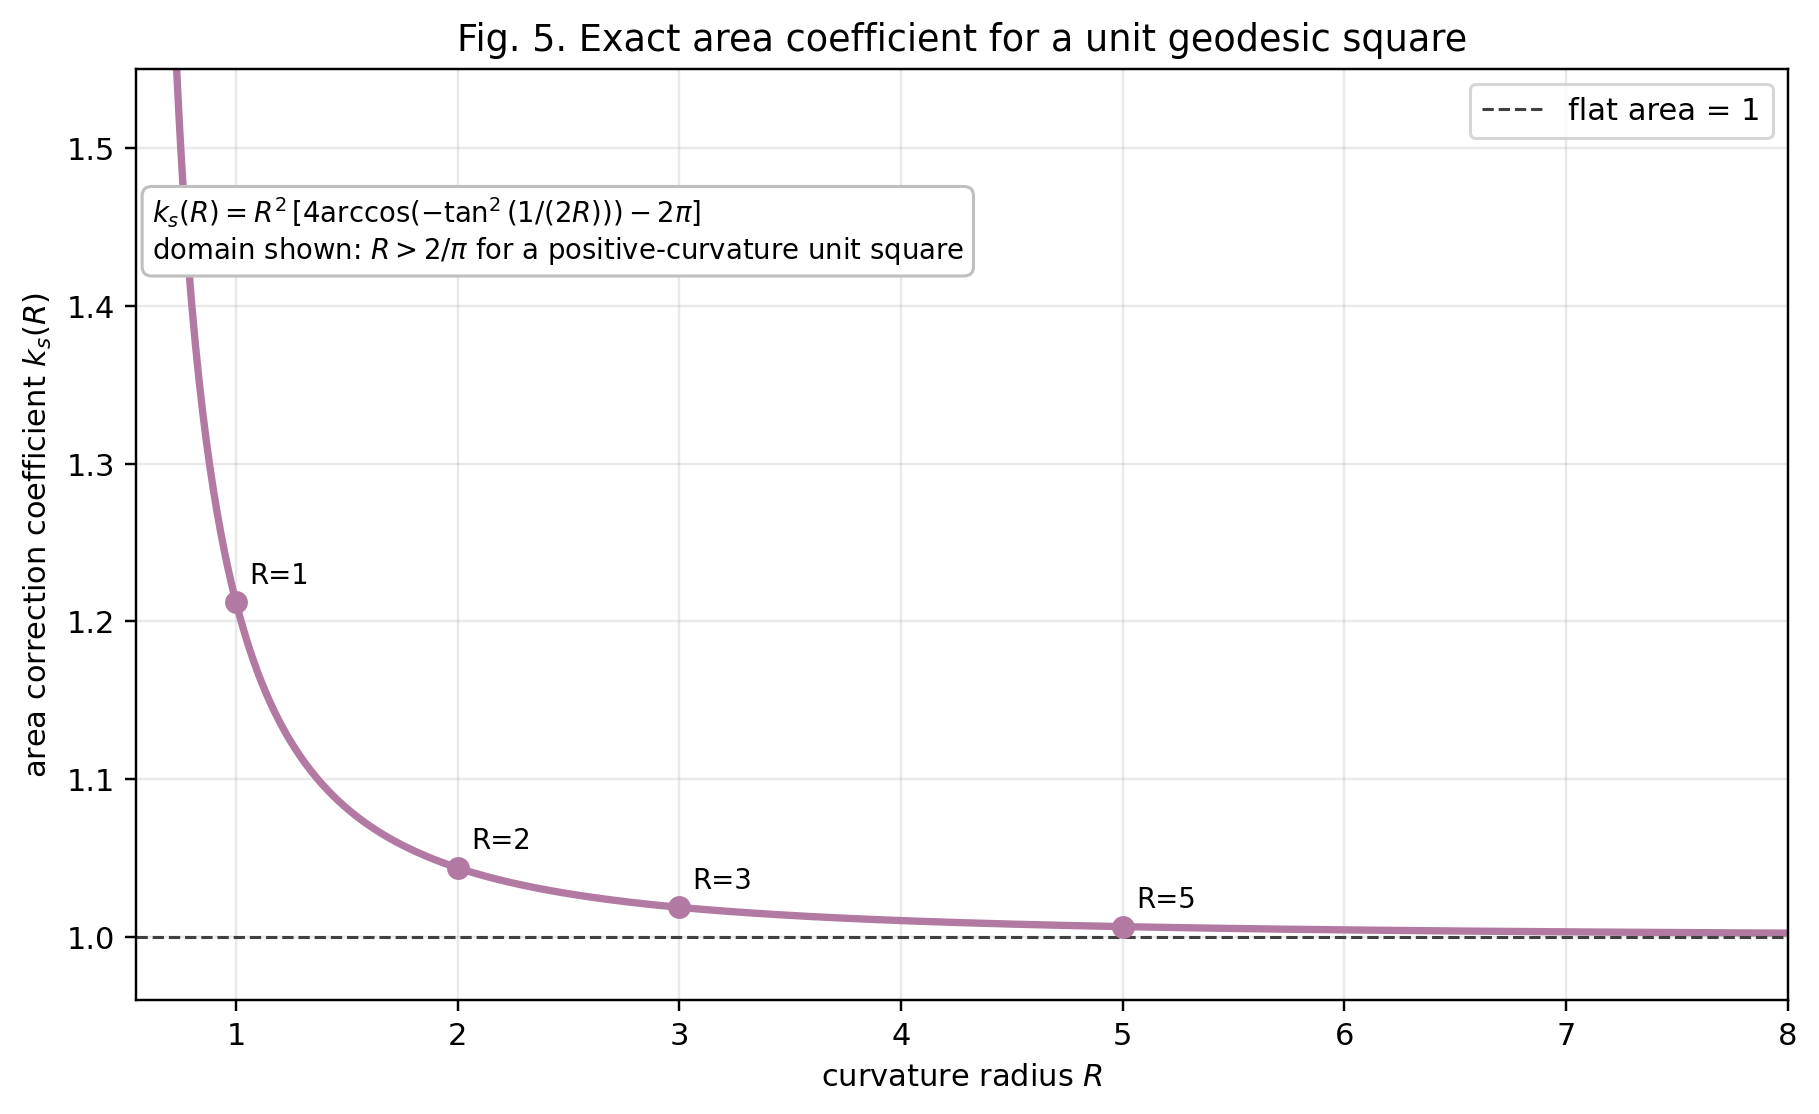
\includegraphics[keepaspectratio,alt={Fig. 5}]{figures/fig05_area_coefficient_ks.png}}
\caption{Fig. 5}
\end{figure}

\textbf{Figure 5.} The area-correction coefficient \(k_s(R)\) of a
geodesic square of side length 1, obtained from the formula of the
self-referenced Paper 0.

\subsubsection{5.4 Test Insertion into the Centrifugal-Type
Model}\label{test-insertion-into-the-centrifugal-type-model}

From the above, one test model readout of the centrifugal-type equation
containing area correction is

\[
a_c^{(R)}=k_s(R)\frac{v^2}{r}.
\]

If a mass \(m\) is externally assigned, then

\[
F_c^{(R)}=m\,k_s(R)\frac{v^2}{r}.
\]

Here \(k_s(R)\) is not an adjustable free parameter. Once the curvature
radius \(R\) is fixed, it is uniquely determined by the geometric
formula of the self-referenced Paper 0.

However, the fact that \(k_s(R)\) is uniquely determined is different
from the claim that it must be inserted into a centrifugal-type equation
in precisely the direction written above. Depending on whether one reads
the quantity as a measure, as a density, as an area, or as an inverse
area, \(k_s(R)\), \(1/k_s(R)\), or another function may appear.

Thus the meaning of this equation is limited. It is not a physical proof
of centrifugal force, but a minimal model in which the classical
centrifugal-type equation is placed in a geometric readout with area
correction. What this paper fixes is only that the centrifugal-type form
contains two directions and, unlike one-dimensional equations, has a
natural entrance for considering area correction.

\begin{center}\rule{0.5\linewidth}{0.5pt}\end{center}

\subsection{6. Geometric Vocabulary: Elliptic, Double-Cone, and
Hyperbolic
Types}\label{geometric-vocabulary-elliptic-double-cone-and-hyperbolic-types}

Quadratic forms appearing under square-quantity readout fall into
several geometric types depending on the signs and the right-hand side.

\[
x^2+y^2=1
\]

is elliptic, and in two dimensions it is a circle.

\[
x^2-y^2=0
\]

is double-cone type, and in a two-dimensional section it is a pair of
lines.

\[
x^2-y^2=1
\]

is hyperbolic.

\begin{figure}
\centering
\pandocbounded{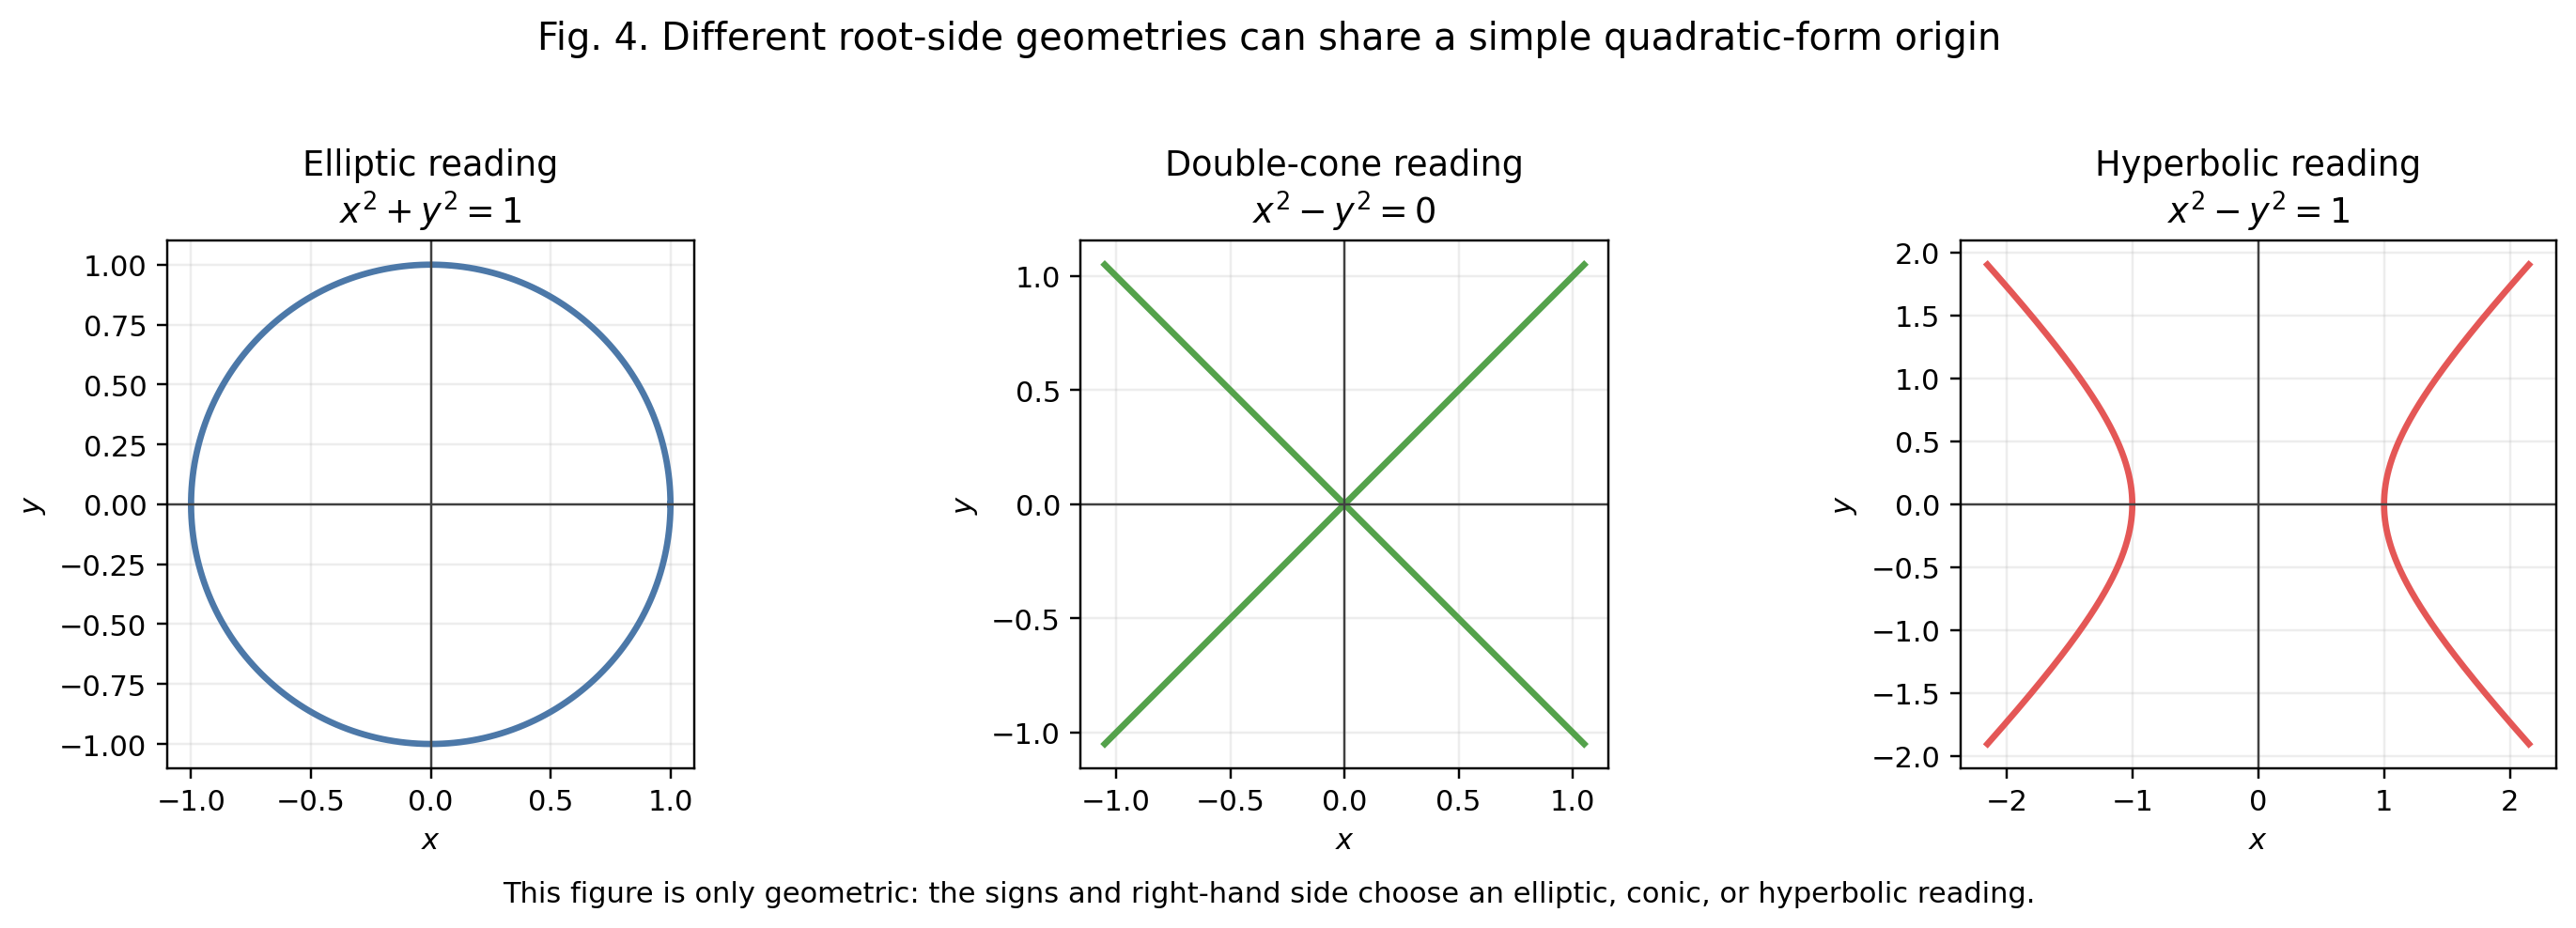
\includegraphics[keepaspectratio,alt={Fig. 4}]{figures/fig04_quadratic_readings.png}}
\caption{Fig. 4}
\end{figure}

\textbf{Figure 4.} Elliptic, double-cone, and hyperbolic readouts appear
from sign choices in the same family of quadratic forms.

This paper uses these not as types of physical space, but as vocabulary
for pure quadratic curves and surfaces appearing on the square-root
side.

\begin{center}\rule{0.5\linewidth}{0.5pt}\end{center}

\subsection{7. Relation to Known Structures and the Scope of This
Paper's
Originality}\label{relation-to-known-structures-and-the-scope-of-this-papers-originality}

\subsubsection{7.1 Known Parts}\label{known-parts}

It is known, in a broad sense, that a positive square-root or square map
relates a simplex to the positive orthant of a sphere.

For example, in information geometry, if one takes

\[
q_i=\sqrt{p_i}
\]

for probability densities \(p_i\), then

\[
\sum_i p_i=1
\]

becomes

\[
\sum_i q_i^2=1.
\]

In this square-root density representation, a probability simplex is
treated as a positive spherical region, and the relation between the
Fisher--Rao metric and spherical geometry is studied.

Therefore, this paper does not claim the square-root correspondence
between a simplex and a positive spherical orthant itself as a new
discovery.

\subsubsection{7.2 The Organizing Principle of This
Paper}\label{the-organizing-principle-of-this-paper}

The possible originality of this paper does not lie in the square map
itself. The square map is an entrance and is close to known structures.
The possible contribution of this paper is the organizing principle that
asks, after the square-quantity readout is adopted, ``where should a
curvature-correction candidate be considered?'' in a dimension-wise
manner.

More concretely, the contribution is the following combination.

\begin{enumerate}
\def\labelenumi{\arabic{enumi}.}
\tightlist
\item
  Instead of probability densities, general square quantities
  \(X_i=x_i^2\) are placed as the basic readout.
\item
  The fact that a curved sum-of-squares constraint becomes a linear
  simplex constraint on the square-quantity side is formulated as
  algebra and geometry without physical interpretation.
\item
  A linear and a quadratic equation placed on the square-quantity side
  are shown to become the uniform-motion and
  uniformly-accelerated-motion forms under positive square-root readout.
\item
  Even when masses and conservation laws are placed, as in a two-body
  collision, no area correction appears as long as the relation is
  closed in one dimension.
\item
  Using the structure from the self-referenced Paper 0 that ``the seat
  of distortion lies at \(d\ge2\)'', relations involving only length are
  separated from relations involving an area cell.
\item
  A centrifugal-type model, in which an area quantity first appears, is
  positioned as the first natural test example for the appearance of
  \(k_s(R)\). However, the way of multiplying by \(k_s(R)\) is not
  claimed to have been uniquely derived as a law of mechanics.
\end{enumerate}

If an existing paper were found that states this entire combination in
the same form, namely square-quantity readout, linear simplexification,
absence of correction in one-dimensional equations, appearance of a
correction candidate in two-dimensional area cells, and connection to
the geodesic-square coefficient \(k_s(R)\) in constant curvature, then
the present paper should be positioned not as a new organizing principle
but as a rediscovery. In the range checked so far, square-root density
representations and Fisher--Rao geometry are close, but no source has
been confirmed that states this dimension-wise organization of
curvature-correction candidates in the same form.

\begin{center}\rule{0.5\linewidth}{0.5pt}\end{center}

\subsection{8. Conclusion}\label{conclusion}

This paper formulated the positive square map

\[
X_i=x_i^2
\]

as a basic readout, and showed that the sum-of-squares constraint

\[
\sum_i x_i^2=E
\]

becomes the linear simplex constraint

\[
\sum_i X_i=E
\]

on the square-quantity side.

From this simple correspondence, the linear equation

\[
X=A T
\]

placed on the square-quantity side becomes, on the positive square-root
side,

\[
x=\sqrt{A}\,t,
\]

and the quadratic equation

\[
X=\frac{1}{2} B T^2
\]

becomes

\[
x=\sqrt{B/2}\,t^2.
\]

These are isomorphic to the classical uniform-motion and
uniformly-accelerated-motion forms, but this paper does not call them
derivations of physical laws.

Also, even if the equations for a two-body perfectly elastic collision
are externally placed, no area correction appears as long as the
equations are closed by one-dimensional velocities alone. This indicates
that the entrance to curvature correction is not ``acceleration'' or
``mass'' itself, but a two-dimensional area quantity.

Finally, in a centrifugal-type model, tangential and radial directions
appear simultaneously, and a natural entrance for considering a
two-dimensional area cell arises. In that case, the exact formula from
the self-referenced Paper 0 gives

\[
k_s(R)
=
R^2
\left[
4\arccos\!\left(-\tan^2\frac{1}{2R}\right)-2\pi
\right].
\]

This coefficient is not an arbitrary adjustment coefficient, but is
defined as the area of a geodesic square of side length 1. However, how
it should be reflected in a centrifugal-type mechanical equation is a
separate issue. This paper only places, as a minimal test model,

\[
a_c^{(R)}=k_s(R)\frac{v^2}{r}.
\]

This is the scope of the paper. Square-quantity readout juxtaposes a
curved sum-of-squares constraint, a linear simplex constraint,
elementary motion forms, and an area-correction coefficient within one
elementary algebraic-geometric flow. Its core is neither to erase
curvature nor to derive area correction from the non-isometry of the
square map. It is to organize, dimension by dimension, the difference
between relations closed by length alone and relations for which a
two-dimensional area cell should be considered.

\begin{center}\rule{0.5\linewidth}{0.5pt}\end{center}

\subsection{References}\label{references}

\subsubsection{Self-reference}\label{self-reference}

\begin{itemize}
\tightlist
\item
  {[}Kihara 2026{]} Noriaki Kihara,
  \href{../波長空間と周波数空間の双対幾何/paper0_geodesic_cell_distortion_en_v1_4.md}{``Paper
  0: Distortion of the Geodesic Unit Cell in Positively-Curved
  Constant-Curvature Space -- Exact Evaluation of Edge, Angle, Area, and
  Volume''}, v1.4, Zenodo DOI 10.5281/zenodo.20684135.
\end{itemize}

\subsubsection{Related References}\label{related-references}

\begin{itemize}
\tightlist
\item
  {[}Saha--Bharath--Kurtek 2017{]} A. Saha, K. Bharath, S. Kurtek,
  \href{https://arxiv.org/abs/1707.09714}{\emph{A Geometric Variational
  Approach to Bayesian Inference}}, arXiv:1707.09714.
\item
  {[}Holbrook--Lan--Streets--Shahbaba 2017{]} A. Holbrook, S. Lan, J.
  Streets, B. Shahbaba,
  \href{https://arxiv.org/abs/1707.03117}{\emph{The nonparametric Fisher
  geometry and the chi-square process density prior}}, arXiv:1707.03117.
\item
  {[}Bauer--Bruveris--Michor 2014{]} M. Bauer, M. Bruveris, P. W.
  Michor, \href{https://arxiv.org/abs/1411.5577}{\emph{Uniqueness of the
  Fisher--Rao metric on the space of smooth densities}},
  arXiv:1411.5577.
\item
  {[}Chern 1944{]} S.-S. Chern,
  \href{https://doi.org/10.2307/1969302}{\emph{A Simple Intrinsic Proof
  of the Gauss--Bonnet Formula for Closed Riemannian Manifolds}}, Annals
  of Mathematics \textbf{45}(4), 747--752 (1944).
\end{itemize}

\end{document}
